\section{Material \& Methods}

\subsection{Data collection}
I collected data on body size of fossil testudinids from the Miocene until recent times. The body size data set includes 30 genera, comprising over 100 fossil species. The majority of the data was obtained from the primary literature (Table \ref{tab:DataFossil}). To find relevant publications, I relied mostly on the references listed in the FosFarBase \citep{Bohme2003b}, the Paleobiology Database (PDBD), and the review by \cite{rhodin2015turtles}.
Furthermore, the FosFarBase provided fossil occurrences of testudinids all over the world, including their exact localities and age (Table \ref{TabS2}\todo{put table only on CD?}, Fig. \ref{fig:mapOc}), which were used to get an overview over the availability of body size data. The FosFarBase (last accessed 23.03.2017) contained 769 testudinid occurrences between the Eocene (33.9 - 56 mya) and the Holocene from 647 localities (Fig. \ref{fig:mapOc}). Of those, 641 occurrences from 534 localities were of relevant Age (Miocene to Holocene). The final body size data set, however, includes 376 data records from 193 localities, of which 106 localities are present in the FosFarBase.


%__________________________________________________________________
 \begin{figure}[htbp]
 	\centering
 	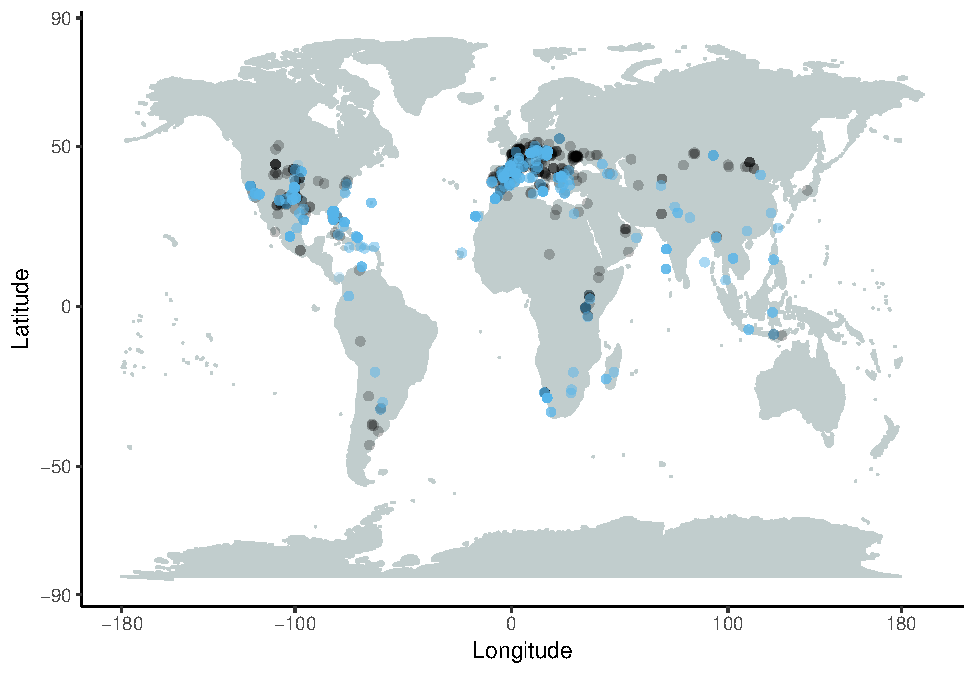
\includegraphics[width=\textwidth]{MA_JJ_files/figure-latex/MapFossilOccurrences-1.pdf}
 	\caption[Map: fossil occurences]{Map displaying all fossil occurrences of testudinids from the Eocene to the Holocene as according to the FosFarBase, with
 		color indicating whether body size data was available (blue) or not (black).}
 	\label{fig:mapOc}
 \end{figure}

For extant taxa, I measured dry material (n = 67) from the collection of the Museum für Naturkunde zu Berlin (MFN). In addition, body size data (n = 173) from the literature was included (Table \ref{tab:DataExtant}).

\subsection{Body size estimation}
Body size is reported as straight carapace length (SCL) in mm. Where SCL was not available from the primary literature, it was estimated (n = 254) either from plastron length (PL) or appendicular elements (Table \ref{tab:DataFossil}). For carapace length estimations based on plastron length, the measurements from the MFN collection material were used to calculate the ratio between SCL and PL. Since the SC/PL ratio was similar for all species (SCL/PL between 0.95 - 1.47)\todo{do I need to provide statistics for that? do I need this sentence at all?}, a single general ratio (SCL/PL = 1.1) was calculated for all testudinids and hence used for the SCL estimations unless stated otherwise (Table \ref{tab:DataFossil}). For estimations based on femora and humeri, the ratios based on data provided by \cite{Hutterer1998} and \cite{Franz2001a}, respectively, were used. A number of publications did not state measurements but instead provided scaled figures of the fossil remains, from which either SCL directly or PL, humeri, or femora lengths for estimating SCL could be measured.

%TO DO: check Franz \& Quitmyer, 2005 again!! (CL regression)

\subsection{Analyses}
All subsequent analyses were performed with R 3.4.1 \citep{RCoreTeam2017}, including the packages dplyr \citep{Wickham2017} to prepare the data for the analysis and ggplot2 \citep{Wickham2009} to create figures. The R package vegan \citep{Oksanen2017} was used to create Sampling Accumulation Curves (most commonly referred to as Species Accumulation Curves), which show the increase in individuals, species or genera per sampling unit and are therefore used to determine if sampling is sufficient or not in terms of covering diversity and richness. 
\todo{explain what species accumulation curves are and give reference}
Since the data set relies on literature, references were used as a sampling unit (x-axis).%and reach a maximum, when no new species/genera are added. 
Sampling Accumulation Curves were created on species as well as genus level, since genera of fossil testudinids are relatively well resolved by now whereas determination on the species level is still somewhat obscure in some cases, because fossil species are frequently based on single individuals that are often fragmentary as well \citep{Brattstrom1961}. Since genera were better sampled than species (Fig. \ref{fig:SACGen}, \ref{fig:SACall} (a) - (b)), all subsequent analysis were performed on the generic level.
Additional Sampling Accumulation Curves for the continents were created (Fig. \ref{fig:SACAll} (c) -  (i)), to check if subsequent analyses could be applied to these subgroups. 
% read Species Accumulation Curve papers + Catalinas paper!
% REWRITE

\subsubsection{Data strucure and statistics}
Histograms and boxplots of the entire data set and several subgroups (fossil vs. modern, insular vs. continental) were created to explore the structure of the data set. General parameters like mean, median, variance, and with the package moments \citep{Komsta2015} skewness and kurtosis were calculated (Table \ref{tab:stats}). The Wilcoxon Rank Sum Test (unpaired data) was used to test for differences between two subgroups. To be able to compare different subgroups, a subsample (1000 repeats) of the respective larger subgroup was taken to compare equal sample sizes. 

%- only used samples > 23.000 mya?!

%__________________________________________________________________
\begin{figure}[htbp]
	\centering
	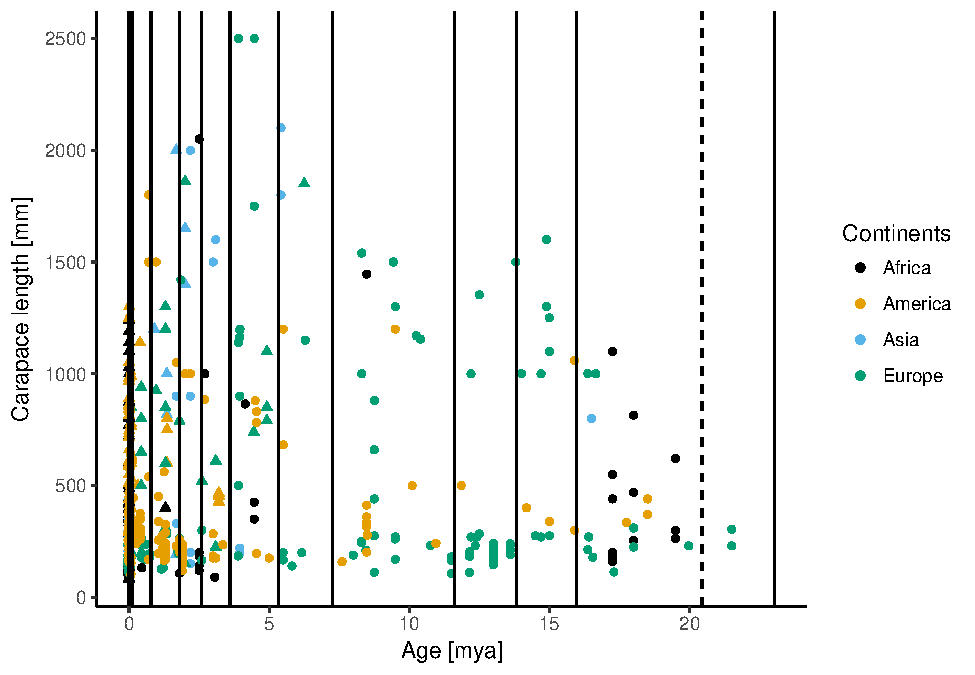
\includegraphics[width=0.8\textwidth]{MA_JJ_files/figure-latex/overviewData-1.pdf}
	\caption[Carapace length over time]{Scatterplot of carapace length over time, indicating insular
		(triangle) and continental (circles) and colour indicating continents.
		Lines indicate stratigraphic stages which were used as time bins, the
		dashed line is the border between the two stages of the Lower Miocene,
		which were consideres as one time bin.}
	\label{fig:bins}
\end{figure}





\subsubsection{Body size trends over time}
To investigate trends in body size over time, the R package paleoTS \citep{Hunt2015a} was used. Data were split into time bins according to stratigraphic stages (Table \ref{tab:bins}, Fig. \ref{fig:bins}), although the two stages of the Lower Miocene were considered as one time bin, because the last bin otherwise would have contained only 2 data records. To prevent sampling bias and because Sampling Accumulation Curves showed that the genus level was well sampled in contrast to species level, the mean SCL per genus was calculated before the timescale analysis. The paleoTS plots were created, wich display the mean trait over time and can be fitted to different evolutionary models: stasis, which ...., generalized random walk (GRW), which .... or unbiased random walk (URW), which..... . The Akaike Weight Criterion (AICc) indicates which model is best supported --> see Catalina's Paper and Hunt's papers


\FloatBarrier
